\section{Design/implementation details}
%More detailed description of how the game/robot controller was designed and implemented including complete class-diagram, description of the implemented classes etc.

\subsection{API on server}

\begin{table}[h]
\begin{tabular}{|p{3.1cm}|p{1.7cm}|p{5cm}|p{3cm}|p{2.5cm}|}
\hline
\textbf{Route}  & \textbf{Request type} & \textbf{Result}                                                & \textbf{Controller} & \textbf{Models} \\ \hline
/play           & POST                  & \{game: game model OR null\}                                  & Matchmaker.js       & Board, Game     \\ \hline
/turn/:username & GET                   & \{username: String, lastMove String\}                                           & Turn.js             & Board, Game     \\ \hline
/fire           & POST                  & \{message: "Ongoing game' OR 'You won',  shipWasHit: Boolean\} & Play.js             & Board, Game     \\ \hline
/cancel         & POST                  & \{username: String\}                                           & Matchmaker.js       & Board, Game     \\ \hline
\end{tabular}
\label{tab:server-routes}
\caption{Table describing the server's implemented routes, affected models and their response.}
\end{table}

% TODO: Add image of classes here

\subsection{Game model (JSON)}
The following list describes the structure of the game object exchanged between the client and the server: 

\label{subsec:gamemodel}
\begin{description}
\item[game:] Object \hfill \
    \begin{description}
    \item player1: String
    \item player2: String
    \item next: String
    \item gameOver: Boolean
    \item lastMove: String
    \item finished: Boolean
    \item [Boards:] Array \hfill \
        \begin{description}
        \item [cells:] Array \hfill \
             \begin{description}
             \item containsShip: Boolean
             \item hasBeenHit: Boolean
             \end{description}
        \end{description}
    \end{description}
\label{game-model}
\end{description}

\subsection{Class Diagrams}

\subsubsection{Server}

\begin{figure}[H]
    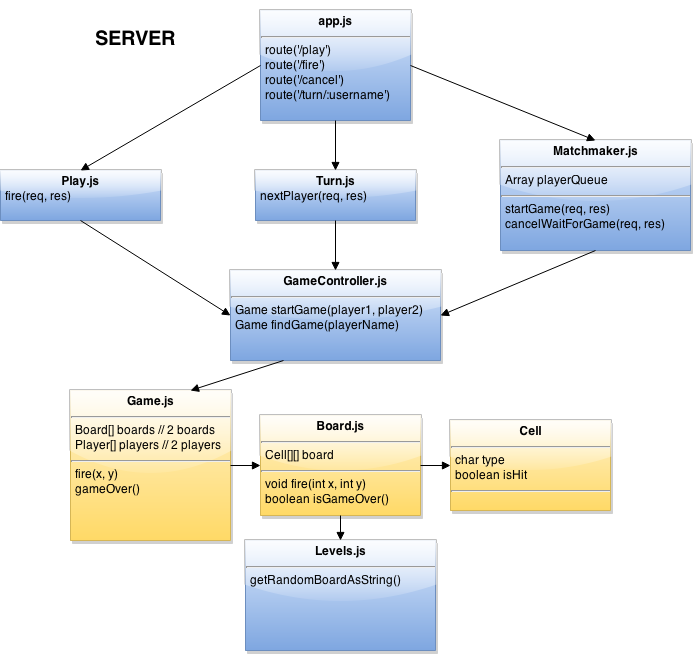
\includegraphics[width=\textwidth]{figs/server_class_diagram.png}
    \caption{Class Diagram of the node.js server. Blue classes are controllers, yellow ones are models.}
    \label{fig:class_diagram_server}
\end{figure}

\subsubsection{Client}

\begin{figure}[H]
    \hspace*{-0.7in}
    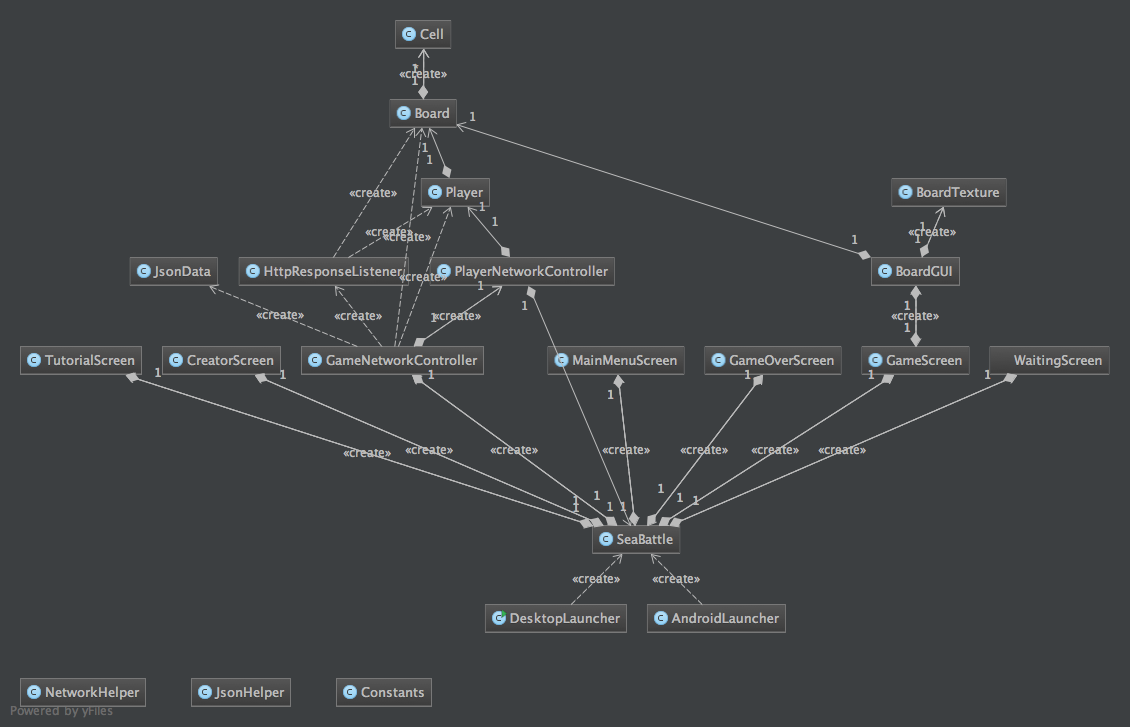
\includegraphics[scale=0.5]{figs/client_class_diagram.png}
    \caption{Class Diagram of the libGDX game}
    \label{fig:class_diagram_client}
\end{figure}



\subsection{Textual description}

\subsubsection{Server}
The server provides four different routes: /play, /fire, /cancel and /turn/:username declared in app.js in the server folder. Every route (see table~\ref{tab:server-routes}) is controlled by a controller that invokes a centralized GameController.js to find and start games.  

When a player wants to play, he sends his username to the play route. If an opponent is already waiting in the queue, the opponent is popped from the queue and a game is created, put in the database, and sent back to the player. Otherwise, the player is put in the queue, and has to regularly poll the /play route to see if a game exists. The maximum size of the queue is always 1. 

To fire, a player sends a username and coordinates to the fire route, which is controlled by the Play controller. The ongoing game is fetched from the database, and a shot will be fired at the opposite player, if it is the current player's turn.

We used the object-relational mapper Sequelize~\cite{sequelize} to handle the connection between our logical models (Game and Board), written in JavaScript, and their representations in our database. Sequelize is initialized in /models/index.js, where the models are loaded and the association between games and boards is set up. While Sequelize can work with several different SQL database management systems, we used PostgreSQL specifically; the authentication details that Sequelize uses to connect to the database, are given through the environment variable DATABASE\_URL, both in production and development.

\subsubsection{Client}
The game is started by the class "SeaBattle", as shown in the class diagram in figure \ref{fig:class_diagram_client}. The different views, that is the classes ending with "screen" in the class diagram, each extends the LibGDX "Screen"-class. These screens has buttons which depend upon the observer-pattern, and which on press executes different actions. It is the "SeaBattle"-class which controls which view is currently shown. The BoardGUI represents a board, and has a grid layout. It uses the local board model as data for the view.

When it comes to networking, the client has two network controllers, namely GameNetworkController and PlayerNetworkController as shown in the class diagram. GameNetworkController sends a request to "/play" (see table \ref{tab:server-routes}), and if the response is a null game object, the client polls "/play" every fifth second to see if an opponent is ready to play. The request is invoked as a TimerTask which is run in a separate thread. 

When a game object is ready, the client build models from JSON game objects which has the format described in subsection~\ref{subsec:gamemodel}. The parsing is done by local models, helped by static helper methods in the class "JSONHelper". The models that are set are instances in PlayerNetworkController. The GUI can then use the models to create graphics, and the fire-method in PlayerNetworkController to send a new network requests. When e.g. a fire-request is sent (described in table \ref{tab:server-routes}). If the request is successful, the client updates the views and local models. This is possible because the game object holds both boards in the first place, and the server request is just meant to see if there's still connectivity and get the move of the opponent.

